\subsection{Strain rate and spin tensor}
\index{velocity gradient}
\index{strain rate}
\index{spin tensor}

The velocity gradient is given in Cartesian coordinates by:
\begin{equation}
\vec\nabla\vec\upnu = 
\left(
\begin{array}{ccc}
\frac{\partial u}{\partial x} & \frac{\partial v}{\partial x} & \frac{\partial w}{\partial x} \\\\
\frac{\partial u}{\partial y} & \frac{\partial v}{\partial y} & \frac{\partial w}{\partial y} \\\\
\frac{\partial u}{\partial z} & \frac{\partial v}{\partial z} & \frac{\partial w}{\partial z} 
\end{array}
\right)
\end{equation}
It can be decomposed into its symmetric and skew-symmetric parts according to:
\begin{equation}
\vec\nabla\vec\upnu = \vec\nabla^s\vec\upnu + \vec\nabla^w\vec\upnu
\end{equation}
The symmetric part is called the strain rate (or rate of deformation):
\begin{equation}
\dot{\bm \epsilon}(\vec \upnu) = \frac{1}{2}\left( \vec\nabla\vec\upnu + \vec\nabla\vec\upnu^T \right)
\end{equation}
The skew-symmetric tensor is called spin tensor (or vorticity tensor):
\begin{equation}
\dot{\bm R}(\vec \upnu) = \frac{1}{2}\left( \vec\nabla\vec\upnu - \vec\nabla\vec\upnu^T \right)
\end{equation}

\begin{remark}
In the mathematical literature a different notation for the strain rate tensor is often used, i.e. 
$D(\vec \upnu)$, such as for instance in \cite{full95}.
\end{remark}



%.............................................
\subsubsection{Compressible Newtonian Fluid}

For the compressible case, ${\bm \sigma}$ 
depends linearly on the strain rate tensor $\dot{\bm \varepsilon}$: 
\begin{equation}
{\bm \sigma} = -p(\rho,T) {\bm 1} + \lambda \; \text{tr} (\dot{\bm \varepsilon}) {\bm 1} + 2\eta \dot{\bm \varepsilon}
\end{equation}
where $p$ is the thermodynamic pressure which is a function of the density $\rho$ and the temperature $T$ (an equation of state is then needed). $\lambda$ and $\eta$ are the coefficients of viscosity. 
We also have:
\begin{equation}
{\bm \sigma} = -p(\rho,T) {\bm 1} + \zeta \; \text{tr} (\dot{\bm \varepsilon}) {\bm 1} + 2\eta \dot{\bm \varepsilon}^d
\end{equation}
where $\zeta=\lambda+2\eta/3$ is the bulk viscosity and $\eta$ is the shear viscosity.



%.............................................
\subsubsection{Incompressible Newtonian Fluid}

In this case the stress tensor is 
\begin{equation}
{\bm \sigma}=-p {\bm 1} + {\bm \tau}
\end{equation}
where $p=-1/3 \; \text{tr} (\bm \sigma)$ and ${\bm \tau}$ is the deviatoric stress tensor:
\begin{equation}
{\bm \tau}=2\eta \dot{\bm \varepsilon}^d
\end{equation}


%------------------------------------------------------------------------
\subsection{The heat transport equation - energy conservation equation}

Let us start from the heat transport equation as shown in Schubert, Turcotte and Olson \cite{scto01}:
\begin{equation}
\rho C_p \frac{DT}{Dt} - \alpha T \frac{Dp}{Dt} = {\vec \nabla} \cdot k {\vec \nabla} T + \Phi + \rho H  
\end{equation}
with $D/Dt$ being the total derivatives so that 
\begin{equation}
\frac{DT}{Dt} = \frac{\partial T}{\partial t} + {\vec \upnu}\cdot {\vec \nabla}T
\quad\quad
\frac{Dp}{Dt} = \frac{\partial p}{\partial t} + {\vec \upnu}\cdot {\vec \nabla}p
\end{equation}
Solving for temperature, this equation is often rewritten as follows:
\begin{mdframed}[backgroundcolor=blue!5]
\begin{equation}
\rho C_p \frac{DT}{Dt} - {\vec \nabla} \cdot k {\vec \nabla} T =  \alpha T \frac{Dp}{Dt} + \Phi + \rho H  
\end{equation}
\end{mdframed}
where $\Phi$ is the shear heating \cite[p287]{reddybook2}. In many publications, $\Phi$ 
is given by $\Phi=\tau_{ij}\partial_j u_i={\bm \tau}:{\vec \nabla}{\vec \upnu}$.

\begin{eqnarray}
\Phi 
&=& \tau_{ij}\partial_j u_i \nonumber\\
&=& 2 \eta \dot{\varepsilon}_{ij}^d\partial_j u_i \nonumber\\
&=& 2 \eta \frac{1}{2}\left( \dot{\varepsilon}_{ij}^d\partial_j u_i + \dot{\varepsilon}_{ji}^d\partial_i u_j \right) \nonumber\\
&=& 2 \eta \frac{1}{2}\left( \dot{\varepsilon}_{ij}^d\partial_j u_i + \dot{\varepsilon}_{ij}^d\partial_i u_j \right) \nonumber\\
&=& 2 \eta  \dot{\varepsilon}_{ij}^d  \frac{1}{2}\left(\partial_j u_i + \partial_i u_j \right) \nonumber\\
&=& 2 \eta  \dot{\varepsilon}_{ij}^d   \dot{\varepsilon}_{ij} \nonumber\\
&=& 2 \eta  \dot{\bm \varepsilon}^d :  \dot{\bm \varepsilon} \nonumber\\
&=& 2 \eta  \dot{\bm \varepsilon}^d : \left( \dot{\bm \varepsilon}^d +\frac{1}{3} ({\vec \nabla}\cdot{\vec \upnu}) {\bm 1} \right)\nonumber\\
&=& 2 \eta  \dot{\bm \varepsilon}^d : \dot{\bm \varepsilon}^d 
+ 2 \eta  \dot{\bm \varepsilon}^d : {\bm 1} ({\vec \nabla}\cdot{\vec \upnu}) \nonumber\\ 
&=& 2 \eta  \dot{\bm \varepsilon}^d : \dot{\bm \varepsilon}^d 
\end{eqnarray}
Finally
\[
\Phi = {\bm \tau}:{\vec \nabla}{\vec \upnu} = 2 \eta  \dot{\bm \varepsilon}^d : \dot{\bm \varepsilon}^d
= 2 \eta \left( (\dot{\varepsilon}_{xx}^d)^2 + (\dot{\varepsilon}_{yy}^d)^2 + 2(\dot{\varepsilon}_{xy}^d)^2 \right)
\]

%------------------------------------------------------------------------
\subsection{The momentum conservation equations} 

Because the Prandlt number is virtually zero in Earth science applications the Navier Stokes 
equations reduce to the Stokes equation:
\begin{equation}
{\vec \nabla}\cdot {\bm \sigma} + \rho {\vec g} = \vec{0}
\end{equation}
Since 
\begin{equation}
{\bm \sigma} = -p {\bm 1} + {\bm \tau}
\end{equation}
it also writes
\begin{equation}
-{\vec \nabla}p + {\vec \nabla}\cdot {\bm \tau} + \rho {\vec g} = \vec{0}
\end{equation}
Using the relationship ${\bm \tau} = 2 \eta \dot{\bm \varepsilon}^d$ we arrive at 
\begin{mdframed}[backgroundcolor=blue!5]
\begin{equation}
-{\vec \nabla}p + {\vec \nabla}\cdot (2 \eta \dot{\bm \varepsilon}^d ) + \rho {\vec g} = \vec{0}
\end{equation}
\end{mdframed}

%------------------------------------------------------------------------
\subsection{The mass conservation equations} 
\index{Solenoidal field} \index{Divergence-free}

The mass conservation equation is given by
\[
\frac{D\rho}{Dt} + \rho {\vec \nabla}\cdot{\vec \upnu} = 0
\]
or, 
\begin{mdframed}[backgroundcolor=blue!5]
\[
\frac{\partial \rho}{\partial t} + {\vec \nabla}\cdot(\rho {\vec \upnu}) = 0
\]
\end{mdframed}
In the case of an incompressible flow, then $\partial \rho/\partial t=0$ and 
${\vec \nabla}\rho=0$, i.e. $D\rho/Dt=0$ and the remaining equation is simply:
\[
{\vec \nabla}\cdot{\vec \upnu} = 0
\]
A vector field that is divergence-free is also called 
solenoidal\footnote{\url{https://en.wikipedia.org/wiki/Solenoidal_vector_field}}.


\subsection{The equations in ASPECT manual}
The following is lifted off the ASPECT manual.
We focus on the system of equations in a $d=2$- or $d=3$-dimensional
domain $\Omega$ that describes the motion of a highly viscous fluid driven
by differences in the gravitational force due to a density that depends on
the temperature. In the following, we largely follow the exposition of this
material in Schubert, Turcotte and Olson \cite{scto01}.

Specifically, we consider the following set of equations for velocity $\mathbf
u$, pressure $p$ and temperature $T$:
\begin{align}
  \label{eq:stokes-1}
  -\vec\nabla \cdot \left[2\eta \left(\dot{\bm \varepsilon}(\vec \upnu)
                                  - \frac{1}{3}(\vec\nabla \cdot \vec \upnu)\mathbf 1\right)
                \right] + \vec\nabla p &=
  \rho \vec g
  &
  & \textrm{in $\Omega$},
  \\
  \label{eq:stokes-2}
  \vec\nabla \cdot (\rho \vec v) &= 0
  &
  & \textrm{in $\Omega$},
  \\
  \label{eq:temperature}
  \rho C_p \left(\frac{\partial T}{\partial t} + \vec \upnu\cdot\vec\nabla T\right)
  - \vec\nabla\cdot k\vec\nabla T
  &=
  \rho H
  \notag
  \\
  &\quad
  +
  2\eta
  \left(\dot\varepsilon(\bm v) - \frac{1}{3}(\vec\nabla \cdot \vec \upnu)\mathbf 1\right)
  :
  \left(\dot\varepsilon(\bm v) - \frac{1}{3}(\vec\nabla \cdot \vec \upnu)\mathbf 1\right)
  \\
  &\quad
  +\alpha T \left( \bm v \cdot \vec\nabla p \right)
  \notag
  \\
  &\quad
  &
  & \textrm{in $\Omega$},
  \notag
\end{align}
where $\dot{\bm \varepsilon}(\vec\upnu) = \frac{1}{2}(\vec\nabla \vec\upnu + \vec\nabla \vec\upnu^T)$ is the symmetric gradient of the velocity (often called the
\textit{strain rate}).%

In this set of equations, \eqref{eq:stokes-1} and \eqref{eq:stokes-2}
represent the compressible Stokes equations in which $\mathbf v=\mathbf
v(\mathbf x,t)$ is the velocity field and $p=p(\mathbf x,t)$ the pressure
field. Both fields depend on space $\mathbf x$ and time $t$. Fluid flow is
driven by the gravity force that acts on the fluid and that is proportional to
both the density of the fluid and the strength of the gravitational pull.

Coupled to this Stokes system is equation \eqref{eq:temperature} for the
temperature field $T=T(\mathbf x,t)$ that contains heat conduction terms as
well as advection with the flow velocity $\mathbf v$. The right hand side
terms of this equation correspond to
\begin{itemize}
\item internal heat production for example due to radioactive decay;
\item friction (shear) heating;
\item adiabatic compression of material;
\end{itemize}

In order to arrive at the set of equations that ASPECT solves, 
we need to 
\begin{itemize}
\item neglect the $\partial p/\partial t$. {\color{red}WHY?}
\item neglect the $\partial \rho / \partial t$ . {\color{red}WHY?}
\end{itemize}
from equations above. 

----------------------------------------

Also, their definition of the shear heating term $\Phi$ is:
\[
\Phi = k_B ({\bm \nabla}\cdot{\bm v})^2 + 2\eta \dot{\bm \varepsilon}^d:\dot{\bm \varepsilon}^d
\]
For many fluids the bulk viscosity $k_B$ is very small and is often taken to be zero, an assumption known
as the Stokes assumption: $k_B=\lambda+2\eta/3=0$. \index{bulk viscosity}
Note that $\eta$ is the dynamic viscosity and $\lambda$ the second viscosity. \index{dynamic viscosity}
\index{second viscosity}
Also, 
\[
{\bm \tau}=2\eta \dot{\bm \varepsilon} + \lambda ({\bm \nabla}\cdot{\bm v}) {\bm 1}
\]
but since $k_B=\lambda+2\eta/3=0$, then $\lambda=-2\eta/3$ so 
\[
{\bm \tau}=2\eta \dot{\bm \varepsilon} -\frac{2}{3}\eta ({\bm \nabla}\cdot{\bm v}) {\bm 1} = 2\eta \dot{\bm \varepsilon}^d
\]







\newpage
%---------------------------------
\subsection{The Boussinesq approximation}
\index{Boussinesq Approximation}

As nicely explained in Spiegel \& Veronis \cite{spve60}: "In the study of problems of thermal convection it is a frequent practice to simplify the basic equations by introducing certain approximations which are attributed to
Boussinesq (1903). The Boussinesq approximations can best be summarized by two
statements: (1) The fluctuations in density which appear with the advent of motion
result principally from thermal (as opposed to pressure) effects. (2) In the equations
for the rate of change of momentum and mass, density variations may be neglected except
when they are coupled to the gravitational acceleration in the buoyancy force."
Note that their paper examines the Boussinesq approximation for compressible fluids.  


[from \aspect{} manual]
The Boussinesq approximation assumes that the density can be
considered constant in all occurrences in the equations with the exception of
the buoyancy term on the right hand side of \eqref{eq:stokes-1}. The primary
result of this assumption is that the continuity equation \eqref{eq:stokes-2}
will now read
\[
{\bm \nabla}\cdot{\bm v} = 0
\]
This implies that the strain rate tensor is deviatoric.
Under the Boussinesq approximation, the equations are much simplified:

\begin{align}
  \label{eq:stokes-1}
  -\nabla \cdot \left[2\eta \dot{\bm \varepsilon}(\bm v)
                \right] + \nabla p &=
  \rho \bm g
  &
  & \textrm{in $\Omega$},
  \\
  \label{eq:stokes-2}
  \nabla \cdot (\rho \bm v) &= 0
  &
  & \textrm{in $\Omega$},
  \\
  \label{eq:temperature}
  \rho_0 C_p \left(\frac{\partial T}{\partial t} + \bm v\cdot\nabla T\right)
  - \nabla\cdot k\nabla T
  &=
  \rho H
  &
  & \textrm{in $\Omega$}
\end{align}
Note that all terms on the rhs of the temperature equations have disappeared, with the exception 
of the source term.


\newpage
%%%%%%%%%%%%%%%%%%%%%%%%%%%%%%%%%%%%%%%%%%%%%%%%%%%%%%%%%%%%%%%%%%%%%%%%%%%%%%%%%%%%%%%%%%55
\subsection{Stokes equation for elastic medium}

What follows is mostly borrowed from Becker \& Kaus lecture notes.

%\begin{tabular}{|l|l|l|}
%\hline
%${\bm u}       $ & displacement vector &   \\
%${\bm \sigma}  $ & full stress tensor  & Pa\\
%${\bm \epsilon}$ & strain tensor       &   \\
%${\bm 1}       $ & unit tensor         &   \\
%${\bm f}       $ & body forces         &   \\
%\hline
%\end{tabular}

The strong form of the PDE that governs force balance in a medium is given by
\[
\vec{\nabla}\cdot{\bm \sigma}  + \vec{f} = \vec{0}
\]
where ${\bm \sigma}$ is the stress tensor and $\vec{f}$ is a body force.

The stress tensor is related to the strain tensor through the generalised 
Hooke's law\footnote{\url{https://en.wikipedia.org/wiki/Hooke's_law}}:
\begin{equation}
\sigma_{ij}=\sum_{kl}C_{ijkl}\epsilon_{kl} 
\qquad
\text{or}
\qquad
{\bm \sigma} = {\bm C} : {\bm \epsilon}
\label{eq:one}
\end{equation}
where ${\bm C}$ is the fourth-order elastic tensor.

Due to the inherent symmetries of ${\bm \sigma}$, ${\bm \epsilon}$, and ${\bm C}$, 
only 21 elastic coefficients of the latter are independent. 
For isotropic media (which have the same physical properties in any direction), ${\bm C}$ 
can be reduced to only two independent numbers (for example the bulk modulus $K$ and the shear modulus $G$ 
that quantify the material's resistance to changes in volume and to shearing deformations, respectively). 

One often then write Eq.~\label{eq:one} as follows:
\begin{equation}
\sigma_{ij}=\lambda \epsilon_{kk} \delta_{ij} + 2\mu \epsilon_{ij}
\quad\quad
or, 
\quad\quad
{\bm \sigma} = \lambda (\vec{\nabla}\cdot\vec{u}) {\bm 1} + 2\mu {\bm \epsilon}   \label{eq:two}
\end{equation}
where $\lambda$ is the Lam\'e parameter and $\mu$ is the shear modulus\footnote{It is also sometimes written $G$}.
The term $\vec{\nabla}\cdot\vec{u}$ is the isotropic dilation.

\index{Lam\'e parameter} \index{shear modulus}

The strain tensor is related to the displacement as follows: \index{strain tensor}
\[
{\bm \epsilon} = \frac{1}{2}(\vec{\nabla}\vec{u} + \vec{\nabla}\vec{u}^T)
\]

The incompressibility (bulk modulus), $K$, is defined as $p=-K \vec{\nabla}\cdot\vec{u}$ 
where $p$ is the pressure with \index{bulk modulus}
\begin{eqnarray}
p&=&-\frac{1}{3} \text{tr}({\bm \sigma}) \nonumber\\
 &=& -\frac{1}{3} [ \lambda (\vec{\nabla}\cdot\vec{u}) \text{tr}[{\bm 1}] + 2 \mu \text{tr}[{\bm \epsilon}]] \nonumber\\
 &=& -\frac{1}{3} [ \lambda (\vec{\nabla}\cdot\vec{u})  3  + 2 \mu  (\vec{\nabla}\cdot\vec{u}) ] \nonumber\\
 &=& -\left[ \lambda + \frac{2}{3} \mu \right] (\vec{\nabla}\cdot\vec{u})  
\end{eqnarray}
so that $K=\lambda+\frac{2}{3}\mu$.

%or
%\[
%\mu=\frac{3K(1-2\nu)}{2(1+\nu)}
%\]


\begin{remark}
Eq. (\ref{eq:one}) and (\ref{eq:two}) are analogous to the ones that one has to solve
in the context of viscous flow using the penalty method. In this case $\lambda$ is the penalty coefficient, 
${\bm u}$ is the velocity, and $\mu$ is then the dynamic viscosity.
\end{remark}

The Lam\'e parameter and the shear modulus are also linked to $\nu$ the poisson ratio, 
and $E$, Young's modulus: \index{Poisson ratio} \index{Young's modulus}
\[
\lambda=\mu\frac{2\nu}{1-2\nu}
=\frac{\nu E}{(1+\nu)(1-2\nu)}
\quad\quad
{\rm with}
\quad\quad
E=2\mu(1+\nu)
\]
The shear modulus, expressed often in GPa, describes the material's response to shear stress.
The poisson ratio describes the response in the direction orthogonal to uniaxial stress.
The Young modulus, expressed in GPa, describes the material's strain response to uniaxial stress in the 
direction of this stress.


%%%%%%%%%%%%%%%%%%%%%%%%%%%%%%%%%%%%%%%%%%%%%%%%%%%%%%%%%%%%%%%%%%55
\newpage
\subsection{The strain rate tensor in all coordinate systems}

The strain rate tensor $\dot{\bm\varepsilon}$ is given by
\begin{equation}
\dot{\bm \varepsilon} = \frac{1}{2}( {\vec \nabla}{\vec \upnu}+ {\vec \nabla}{\vec \upnu}^T) 
\end{equation}

%.....................................
\subsubsection{Cartesian coordinates}
\begin{eqnarray}
\dot\varepsilon_{xx} &=& \frac{\partial u}{\partial x} \\
\dot\varepsilon_{yy} &=& \frac{\partial v}{\partial y} \\
\dot\varepsilon_{zz} &=& \frac{\partial w}{\partial z} \\
\dot\varepsilon_{yx} =
\dot\varepsilon_{xy} &=& \frac{1}{2} \left( \frac{\partial u}{\partial y} + \frac{\partial v}{\partial x}  \right)\\
\dot\varepsilon_{zx} =
\dot\varepsilon_{xz} &=& \frac{1}{2} \left( \frac{\partial u}{\partial z} + \frac{\partial w}{\partial x}  \right)\\
\dot\varepsilon_{zy} =
\dot\varepsilon_{yz} &=& \frac{1}{2} \left( \frac{\partial v}{\partial z} + \frac{\partial w}{\partial y}  \right)
\end{eqnarray}

%.....................................
\subsubsection{Polar coordinates}

\begin{eqnarray}
\dot\varepsilon_{rr} &=& \frac{\partial v_r}{\partial r} \\
\dot\varepsilon_{\theta\theta} &=& \frac{v_r}{r} + \frac{1}{r} \frac{\partial v_\theta}{\partial \theta}  \\
\dot\varepsilon_{\theta r} =
\dot\varepsilon_{r\theta} &=& \frac{1}{2} \left(   \frac{\partial v_\theta}{\partial r} - \frac{v_\theta}{r} 
+\frac{1}{r} \frac{\partial v_r}{\partial \theta}  \right) 
\end{eqnarray}

%.....................................
\subsubsection{Cylindrical coordinates}

\begin{eqnarray}
\dot\varepsilon_{rr} &=& \frac{\partial v_r}{\partial r} \\
\dot\varepsilon_{\theta\theta} &=& \frac{v_r}{r} + \frac{1}{r} \frac{\partial v_\theta}{\partial \theta}  \\
\dot\varepsilon_{\theta r} =
\dot\varepsilon_{r\theta} &=& \frac{1}{2} \left(   \frac{\partial v_\theta}{\partial r} - \frac{v_\theta}{r} 
+\frac{1}{r} \frac{\partial v_r}{\partial \theta}  \right)\\
\dot\varepsilon_{zz} &=& \frac{\partial w}{\partial z} \\
\dot{\varepsilon}_{rz} = \dot{\varepsilon}_{zr} &=& \frac{1}{2}\left(   \right) \\
\dot{\varepsilon}_{\theta z} = \dot{\varepsilon}_{z \theta} &=& \frac{1}{2}\left( \frac{1}{r} \frac{\partial w}{\partial \theta} + \frac{\partial v_\theta}{\partial z}  \right) \\
\end{eqnarray}
 
CHECK AND HOMOGENIZE NOTATIONS



http://eml.ou.edu/equation/FLUIDS/STRAIN/STRAIN.HTM

%.....................................
\subsubsection{Spherical coordinates}

\begin{eqnarray}
\dot\varepsilon_{rr} &=& \frac{\partial v_r}{\partial r} \\
\dot\varepsilon_{\theta\theta} &=& \frac{v_r}{r} + \frac{1}{r} \frac{\partial v_\theta}{\partial \theta}  \\
\dot\varepsilon_{\phi\phi} &=& \frac{1}{r \sin\theta} \frac{\partial v_\phi}{\partial \phi} \\
\dot\varepsilon_{\theta r} =
\dot\varepsilon_{r\theta}   &=& \frac{1}{2} \left( r \frac{\partial}{\partial r} (\frac{v_\theta}{r} ) 
+\frac{1}{r} \frac{\partial v_r}{\partial \theta} \right) \\
\dot\varepsilon_{\phi r} =
\dot\varepsilon_{r\phi}      &=&  \frac{1}{2} \left(  \frac{1}{r \sin\theta} \frac{\partial v_r}{\partial \phi} 
+ r \frac{\partial }{\partial r} (\frac{v_\phi}{r}) \right)  \\
\dot\varepsilon_{\phi \theta} =
\dot\varepsilon_{\theta\phi} &=& \frac{1}{2} \left( \frac{\sin \theta}{r} \frac{\partial }{\partial \theta} (\frac{v_\phi}{\sin\theta}) + \frac{1}{r \sin\theta} \frac{\partial v_\theta}{\partial \phi}    \right) 
\end{eqnarray}



\newpage
%-------------------------------
\subsection{Boundary conditions}

%wiki
In mathematics, the Dirichlet (or first-type) 
boundary condition is a type of boundary condition, named after Peter Gustav Lejeune Dirichlet.
When imposed on an ODE or PDE, it specifies the values that a solution needs 
to take on along the boundary of the domain.
Note that a Dirichlet boundary condition may also be referred to as a fixed boundary condition. 

The Neumann (or second-type) boundary condition is a type of boundary condition, 
named after Carl Neumann. When imposed on an ordinary or a partial differential equation, 
the condition specifies the values in which the derivative of a solution is 
applied within the boundary of the domain.

It is possible to describe the problem using other boundary conditions: 
a Dirichlet boundary condition specifies the values of the solution itself 
(as opposed to its derivative) on the boundary, whereas the Cauchy boundary condition, mixed boundary condition and Robin boundary condition are all different types of combinations of the Neumann and Dirichlet boundary conditions.

\index{Dirichlet boundary condition}
\index{Neumann boundary condition}





%....................................
\subsubsection{The Stokes equations}

You may find the following terms in the computational geodynamics literature:

\begin{itemize}
\item { free surface}: this means that no force is acting on the surface, i.e. ${\bm \sigma}\cdot {\vec n}={\vec 0}$. It is usually used on the top boundary of the domain and allows for topography evolution.
\item { free slip}: ${\vec \upnu}\cdot \vec n = 0$ and $({\bm \sigma}\cdot{\vec n})\times {\vec n}={\vec 0}$. This condition ensures a frictionless flow parallel to the boundary where it is prescribed.
\item { no slip}: this means that the velocity (or displacement) is exactly zero on the boundary, i.e. ${\vec \upnu}={\vec 0}$.
\item { prescribed velocity}: ${\vec \upnu}={\vec \upnu}_{bc}$
\item stress b.c.: 
\item open .b.c.: see fieldstone 29. 
\end{itemize}

%....................................
\subsubsection{The heat transport equation}

There are two types of boundary conditions for this equation: temperature boundary conditions (Dirichlet boundary conditions) and heat flux boundary conditions (Neumann boundary conditions). 

\newpage
%------------------------------------------
\subsection{Meaningful physical quantities}

\begin{itemize}
\item \underline{Velocity} $\vec \upnu (\text{m/s})$: This is a vector quantity and both magnitude and direction are needed to define it. It is the rate of change of position with respect to a frame of reference.
\item \underline{Root mean square velocity} $\upnu_{rms} (\text{m/s})$: 
\begin{equation}
\upnu_{rms} = \left ( \frac{\int_\Omega |{\vec \upnu}|^2 \;  d \Omega}{\int_\Omega d\Omega }  \right )^{1/2}
=\left ( \frac{1}{V_\Omega} \int_\Omega |{\vec \upnu}|^2 \;  d \Omega \right )^{1/2} \label{eqVrms}
\end{equation}
\begin{remark}
$V_\Omega$ is usually computed numerically at the same time $\upnu_{vrms}$ is computed.
\end{remark}
In Cartesian coordinates, for a cuboid domain of size $Lx\times L_y \times Lz$, 
the $\upnu_{rms}$ is simply given by:
\begin{equation}
\upnu_{rms}  = \left ( \frac{1}{L_xL_yL_z} \int_0^{L_x}\int_0^{L_y}\int_0^{L_z} 
(u^2 + v^2 + w^2) dxdydz  \right )^{1/2}
\end{equation}
In the case of an annulus domain, although calculations are carried out 
in Cartesian coordinates, it makes sense
to look at the radial velocity component $\upnu_r$ and the tangential velocity 
component $\upnu_\theta$, and their respective
root mean square averages:
\begin{equation}
\upnu_r|_{rms}  =\left ( \frac{1}{V_\Omega} \int_\Omega v_r^2 \;  d \Omega \right )^{1/2} \label{eqVrVrms}
\end{equation}
\begin{equation}
\upnu_\theta|_{rms}  = \left ( \frac{1}{V_\Omega} \int_\Omega v_\theta^2 \;  d \Omega \right )^{1/2} \label{eqThetaVrms}
\end{equation}


\item \underline{Pressure} $p (\text{Pa})$:
\item \underline{Stress tensor} ${\bm \sigma}$ (Pa): \index{Stress Tensor}
\item \underline{Strain tensor} ${\bm \varepsilon}$ (dimensionless): \index{Strain tensor}
\item \underline{Strain rate tensor} $ \dot{\bm \varepsilon} (\text{s}^{-1}$): \index{Strain rate tensor}
\item \underline{Rayleigh number} $Ra$ (X): \index{Rayleigh Number}
It is a dimensionless number that expresses the	ratio of the driving forces to the opposing forces.
The buoyancy force comes from the volumetric thermal expansion while the viscous forces and 
the heat diffusivity oppose convection (the latter one smoothes out thermal gradients). 

The Rayleigh number for convection driven by a constant temperature hot base and a cold surface
in a domain of thickness $D$ is:
\[
Ra 
= \frac{\rho_0 g \alpha D^3 }{\eta \kappa}  \cdot  \Delta T
= \frac{\rho_0^2 C_p g \alpha D^3 \Delta T}{\eta k}
\]
The Rayleigh number for convection driven by a hot base (constant basal heat flow $q_b$)
and a colder surface is:
\[
Ra = \frac{\rho_0 g \alpha D^3}{\eta \kappa } \cdot  \frac{q_b D}{k}
\]  
The Rayleigh number for convection driven by internal heating $H$ (production per cubic meter) is:
\[
Ra = \frac{\rho_0 g \alpha D^3}{\eta \kappa} \cdot  \frac{H D^2}{k }
\]
The Rayleigh number for convection driven by both basal heat flow and internal heating is:	
\[
Ra = \frac{\rho_0 g \alpha D^3}{\eta \kappa} \cdot  \frac{q_b D + H D^2}{k }
\]
For convection to occur, the Rayleigh number must be larger than the so-called critical 
Rayleigh number, which ranges from 600 to 3000 (it depends on the boundary conditions and the 
geometry).
\index{Critical Rayleigh Number}


\item \underline{Prandtl number} $Pr$ (X): \index{Prandtl Number} It is named after the German physicist 
Ludwig Prandtl and is defined as the ratio of momentum diffusivity to thermal diffusivity. It is given as: 
\[
Pr = \frac{\text{momentum diffusivity}}{\text{thermal diffusivity}} = \frac{\eta/\rho}{k/(\rho C_p)}= \frac{\eta C_p}{k}
\]
For Earth materials, we have $Pr \sim (10^{21} 1000)/3 >> 1$, which means that momentum diffusivity dominates.


\item \underline{Nusselt number} $N_u$ (X): \index{Nusselt Number}  the Nusselt number (Nu) is the ratio of convective to conductive heat transfer across (normal to) the boundary. The conductive component is measured under the same conditions as the heat convection but with a (hypothetically) stagnant (or motionless) fluid.

In practice the Nusselt number Nu of a layer (typically the mantle of a planet) is defined as follows:
\begin{equation}
\text{Nu} = \frac{q}{q_c}
\end{equation} 
where $q$ is the heat transferred by convection while $q_c=k \Delta T /D$ 
is the amount of heat that would be conducted through a layer of
thickness $D$ with a temperature difference $\Delta T$ across it with 
$k$ being the thermal conductivity.

For 2D Cartesian systems of size ($L_x$,$L_y$) the Nu is computed \cite{blbc89}
\[
\text{Nu} = 
 \frac{\frac{1}{L_x}\int_{0}^{L_x} k \frac{\partial T}{\partial y}(x,y=L_y) dx }
{-\frac{1}{L_x}\int_0^{L_x} k T(x,y=0) /L_y dx}
=-L_y \frac{\int_{0}^{L_x} \frac{\partial T}{\partial y}(x,y=L_y) dx }{\int_0^{L_x} T(x,y=0) dx}
\]
i.e. it is the mean surface temperature gradient
over the mean bottom temperature.

\todo[inline]{finish. not happy with definition. Look at literature}

Note that in the case when no convection takes place then the measured heat flux at the top is 
the one obtained from a purely conductive profile which yields Nu=1.

Note that a relationship Ra $\propto$ Nu$^\alpha $ exists between the Rayleigh number Ra and the Nusselt number Nu in convective systems, see \cite{wodd09} and references therein. 

Turning now to cylindrical geometries with inner radius $R_1$ and outer radius $R_2$, we define $f=R_1/R_2$. A small value of $f$ corresponds to a high
degree of curvature. We assume now that $R_2-R_1=1$, so that $R_2=1/(1-f)$ and $R_1=f/(1-f)$. 
Following \cite{jarv93}, the Nusselt number at the inner and outer boundaries are:
\begin{equation}
\boxed{
\text{Nu}_{inner} = \frac{f \ln f}{1-f} \frac{1}{2\pi} \int_0^{2\pi} \left( \frac{\partial T}{\partial r} \right)_{r=R_1} d\theta
}
\label{eqNuAnnIn}
\end{equation}
\begin{equation}
\boxed{
\text{Nu}_{outer} = \frac{\ln f}{1-f} \frac{1}{2\pi} \int_0^{2\pi} \left( \frac{\partial T}{\partial r} \right)_{r=R_2} d\theta
}
\label{eqNuAnnOut}
\end{equation}

Note that a conductive geotherm in such an annulus between temperatures $T_1$ and $T_2$ is given by 
\[
T_c(r)=\frac{\ln (r/R_2)}{\ln(R_1/R_2)} = \frac{\ln(r(1-f))}{\ln f}
\]
so that 
\[
\frac{\partial T_c}{\partial r} = \frac{1}{r}\frac{1}{\ln f} 
\]
We then find:
\begin{eqnarray}
\text{Nu}_{inner} 
&=& \frac{f \ln f}{1-f} \frac{1}{2\pi} \int_0^{2\pi} \left( \frac{\partial T_c}{\partial r} \right)_{r=R_1} d\theta
= \frac{f \ln f}{1-f} \frac{1}{R_1}\frac{1}{\ln f} 
= 1 \\
\text{Nu}_{outer} 
&=& \frac{\ln f}{1-f} \frac{1}{2\pi} \int_0^{2\pi} \left( \frac{\partial T_c}{\partial r} \right)_{r=R_2} d\theta 
= \frac{\ln f}{1-f} \frac{1}{R_2}\frac{1}{\ln f} = 1 
\end{eqnarray}
As expected, the recovered Nusselt number at both boundaries is exactly 1 when the temperature field is
given by a steady state conductive geotherm.

\todo[inline]{derive formula for Earth size R1 and R2}

 
\item \underline{Temperature} (K):
\item \underline{Viscosity} (Pa.s):
\item \underline{Density} (kg/m$^3$):
\item \underline{Heat capacity} $C_p$ ($J.K^{-1}$): It is the measure of the heat energy required to increase the 
temperature of a unit quantity of a substance by unit degree. Note that the specific heat capacity $c_P$ of a 
substance is the heat capacity of a sample of the substance divided by the mass of the sample, with units $J\cdot K\cdot kg^{-1}$.
\item \underline{Heat conductivity}, or thermal conductivity $k$ ($W.m^{-1}.K^{-1}$). It is the property of a material that indicates its ability to conduct     heat. It appears primarily in Fourier's Law for heat conduction.
Note that it is a function of temperature, especially in mantle convection settings \cite{mika13}. See also \cite{boca99} and refs therein.

\item \underline{Heat diffusivity}: $\kappa=k/(\rho C_p)$ ($m^2.s^{-1}$). Substances with high thermal diffusivity rapidly adjust their temperature to that of their surroundings, because they 
conduct heat quickly in comparison to their volumetric heat capacity or 'thermal bulk'.
\item \underline{thermal expansion} $\alpha$ (K$^{-1}$): it is the tendency of a matter to change in volume in response to a change in temperature. Note that it is a function of temperature, especially in mantle convection settings \cite{mika13}.

\item \underline{Urey Ratio}: mantle heat production divided by heat loss) is a key constraint for thermal history models. Recent Urey ratio estimates are in the range of 0.21–0.49. \cite{lecm11}

\end{itemize}


\todo[inline]{check aspect manual The 2D cylindrical shell benchmarks by Davies et al. 5.4.12}


%------------------------------------------------------
\subsection{Principal stress} \label{sec:princ_stress}

\index{Maximum Shear Stress} \index{Principal Stress}

As seen before (see Section~\ref{sec:stresstensor}) 
the stress tensor is a symmetric $3\times3$ real matrix, and linear algebra tells us that it 
therefore has three mutually orthogonal unit-length eigenvectors $\vec{n}_{1}$, $\vec{n}_{2}$, 
$\vec{n}_{3}$ and three real eigenvalues $\lambda _{1},\lambda _{2},\lambda _{3}$ 
such that ${\bm \sigma}\cdot \vec{n}_i=\lambda_{i} \vec{n}_{i}$.

%from wiki stress 
As a consequence, in a coordinate system with axes $\vec{n}_{1},\vec{n}_{2},\vec{n}_{3}$, 
the stress tensor is a diagonal matrix, and has only the three normal components $\lambda _{1},\lambda _{2},\lambda _{3}$
i.e. the principal stresses. If the three eigenvalues are equal, the stress is an isotropic compression or tension, always perpendicular to any surface, there is no shear stress, and the tensor is a diagonal matrix in any coordinate frame.

\subsubsection{In two dimensions}

We are looking for the stress tensor eigenvector vector $\vec{n}=(n_x,n_y)$ associated to the
eigenvalue $\lambda$ such that 
\[
\left(
\begin{array}{cc}
\sigma_{xx} & \sigma_{xy} \\
\sigma_{xy} & \sigma_{yy} 
\end{array}
\right)
\cdot
\left(
\begin{array}{c}
n_x \\ n_y
\end{array}
\right)
=
\lambda
\left(
\begin{array}{c}
n_x \\ n_y
\end{array}
\right)
\]
or,
\[
\left(
\begin{array}{cc}
\sigma_{xx} & \sigma_{xy} \\
\sigma_{xy} & \sigma_{yy} 
\end{array}
\right)
\cdot
\left(
\begin{array}{c}
n_x \\ n_y
\end{array}
\right)
-
\left(
\begin{array}{cc}
\lambda & 0 \\ 
0 & \lambda 
\end{array}
\right)
\cdot
\left(
\begin{array}{c}
n_x \\ n_y
\end{array}
\right)
= \vec{0}
\]
i.e.,
\[
\left(
\begin{array}{cc}
\sigma_{xx}-\lambda  & \sigma_{xy} \\
\sigma_{xy} & \sigma_{yy} -\lambda 
\end{array}
\right)
\cdot
\left(
\begin{array}{c}
n_x \\ n_y
\end{array}
\right)
= \vec{0}
\]

which yields
\[
(\sigma_{xx}-\lambda)(\sigma_{yy}-\lambda)-\sigma_{xy}^2 =0
\]
or, 
\[
\lambda^2 - (\sigma_{xx}+\sigma_{yy}) \lambda   + (\sigma_{xx}\sigma_{yy}-\sigma_{xy}^2) =0
\]
The discriminant $\Delta$ is 
\begin{eqnarray}
\Delta 
&=& (\sigma_{xx}+\sigma_{yy})^2-4(\sigma_{xx}\sigma_{yy}-\sigma_{xy}^2)  \nn\\
&=& (\sigma_{xx}-\sigma_{yy})^2 +4\sigma_{xy}^2  \nn
\end{eqnarray}
The roots are given by:
\begin{eqnarray}
\lambda_\pm 
&=& \frac{ (\sigma_{xx}+\sigma_{yy}) \pm \sqrt{ (\sigma_{xx}-\sigma_{yy})^2 +4\sigma_{xy}^2 } }{2} \nn\\
&=& \frac{ \sigma_{xx}+\sigma_{yy}}{2} \pm \sqrt{ \left(\frac{\sigma_{xx}-\sigma_{yy}}{2}\right)^2 +\sigma_{xy}^2 } \nn\\
\end{eqnarray}
The two principal stresses are then:
\begin{eqnarray}
\sigma_1 &=& \frac{ \sigma_{xx}+\sigma_{yy}}{2} + \sqrt{ \left(\frac{\sigma_{xx}-\sigma_{yy}}{2}\right)^2 +\sigma_{xy}^2 } \nn\\
\sigma_2 &=& \frac{ \sigma_{xx}+\sigma_{yy}}{2} - \sqrt{ \left(\frac{\sigma_{xx}-\sigma_{yy}}{2}\right)^2 +\sigma_{xy}^2 } \nn\\
\end{eqnarray}
with the convention $\sigma_1>\sigma_2$.
The maximum shear stress is defined as one-half the difference between the two principal 
stresses 
\[
\tau_{\text max}=
\frac{\sigma_1-\sigma_2}{2}
=\sqrt{ \left(\frac{\sigma_{xx}-\sigma_{yy}}{2}\right)^2 +\sigma_{xy}^2 } 
\]

The eigenvector $\vec{n}_1$ corresponding to $\sigma_1$ is obtained by solving 
\[
{\bm \sigma}\cdot \vec{n}_1 = \sigma_1 \vec{n}_1
\]
and same for the other eigenvalue/vector:
\[
{\bm \sigma}\cdot \vec{n}_2 = \sigma_2 \vec{n}_2
\]
Each is a system of two equations with two unknowns. These are not difficult to solve, 
but can prove cumbersome. Note that linear algebra tells us that $\vec{n}_1\cdot\vec{n}_2=0$, 
i.e. the eigenvectors form a basis of $\mathbb{R}^2$.

This is the reason why often people go another route. One can ask the question: what is the 
value of the angle $\theta_p$ which, if used to perform a rotation of the axis system, yields 
a stress tensor that is diagonal, with the principal stresses on the diagonal?
 
\begin{center}
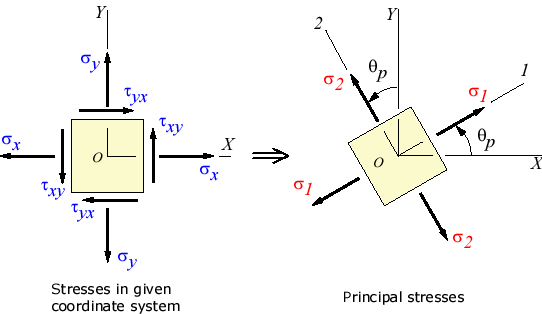
\includegraphics[width=8cm]{images/princ_stress/PrincipalStress}\\
{\scriptsize Taken from \url{https://www.efunda.com/formulae/solid_mechanics/mat_mechanics/plane_stress_principal.cfm}}
\end{center}
 
The rotation matrix is 
\[
{\bm R}=
\left(
\begin{array}{cc}
\cos\theta_p & -\sin\theta_p \\
\sin\theta_p & \cos\theta_p
\end{array}
\right)
\]
and the image of ${\bm \sigma}$ by means of the axis rotation is 
${\bm \sigma}'= {\bm R}\cdot {\bm \sigma}\cdot {\bm R}^{-1}$, i.e.
\begin{eqnarray}
{\bm \sigma}' 
&=&
\left(
\begin{array}{cc}
\cos\theta_p & -\sin\theta_p \\
\sin\theta_p & \cos\theta_p
\end{array}
\right)
\cdot
\left(
\begin{array}{cc}
\sigma_{xx} & \sigma_{xy} \\
\sigma_{xy} & \sigma_{yy} 
\end{array}
\right)
\cdot
\left(
\begin{array}{cc}
\cos\theta_p & \sin\theta_p \\
-\sin\theta_p & \cos\theta_p
\end{array}
\right) \nn\\
&=&\left(
\begin{array}{cc}
\cos\theta_p & -\sin\theta_p \\
\sin\theta_p & \cos\theta_p
\end{array}
\right)
\cdot
\left(
\begin{array}{cc}
\sigma_{xx} \cos\theta_p - \sigma_{xy} \sin\theta_p  &
\sigma_{xx} \sin\theta_p + \sigma_{xy} \cos\theta_p  \\
\sigma_{xy} \cos\theta_p - \sigma_{yy} \sin\theta_p & 
\sigma_{xy} \sin\theta_p + \sigma_{yy} \cos\theta_p 
\end{array}
\right) \nn\\
&=&
\left(
\begin{array}{cc}
\dots & 
\cos\theta_p(\sigma_{xx} \sin\theta_p + \sigma_{xy} \cos\theta_p )-
\sin\theta_p(\sigma_{xy} \sin\theta_p + \sigma_{yy} \cos\theta_p ) \\
\dots & \dots 
\end{array}
\right) \nn 
\end{eqnarray}
In the matrix above I have only computed the off diagonal term since 
we are actually looking for $\theta_p$ such that $\sigma_{xy}'=0$, or
\begin{eqnarray}
\cos\theta_p(\sigma_{xx} \sin\theta_p + \sigma_{xy} \cos\theta_p )-
\sin\theta_p(\sigma_{xy} \sin\theta_p + \sigma_{yy} \cos\theta_p ) &=& 0 \nn\\
\sin\theta_p \cos\theta_p (\sigma_{xx}-\sigma_{yy}) + ( \cos^2\theta_p -\sin^2\theta_p )\sigma_{xy} &=& 0 \nn 
\end{eqnarray}
and then 
\[
\frac{ \sin\theta_p \cos\theta_p}{ \cos^2\theta_p -\sin^2\theta_p }
= \frac{\sigma_{xy}}{ \sigma_{xx}-\sigma_{yy} }
\]
The left hand term is actually a trigonometric 
identity\footnote{\url{https://en.wikipedia.org/wiki/List_of_trigonometric_identities}}:
\[
\frac{ \sin\theta_p \cos\theta_p}{ \cos^2\theta_p -\sin^2\theta_p } = \frac{1}{2} \tan 2\theta_p
\]
and finally:
\[
\tan 2\theta_p = \frac{ 2\sigma_{xy}}{ \sigma_{xx}-\sigma_{yy} }
\qquad
\text{or}
\qquad
\theta_p = \frac{1}{2} \tan^{-1} \frac{ 2\sigma_{xy}}{ \sigma_{xx}-\sigma_{yy} }
\]
Once $\theta_p$ has been found the other direction is given by $\theta_p +\pi/2$.

\vspace{.5cm}

\underline{Example}: Let us start with 
\[
{\bm \sigma} = 
\left(
\begin{array}{cc}
a & 0 \\
0 & b
\end{array}
\right)
\]
then $\tan 2\theta_p = 0$, and then $\theta_p=0$. The principal directions are the horizontal and 
vertical directions, i.e. the Cartesian axis system, which is consistent.

%...................................... 
\subsubsection{In three dimensions}

We are looking for the stress tensor eigenvector vector $\vec{n}=(n_x,n_y,n_z)$ associated to the
eigenvalue $\lambda$ such that 
\[
\left(
\begin{array}{ccc}
\sigma_{xx} & \sigma_{xy} & \sigma_{xz} \\
\sigma_{xy} & \sigma_{yy} & \sigma_{yz} \\
\sigma_{xz} & \sigma_{yz} & \sigma_{zz}
\end{array}
\right)
\cdot
\left(
\begin{array}{c}
n_x \\ n_y \\ n_z
\end{array}
\right)
=
\lambda
\left(
\begin{array}{c}
n_x \\ n_y \\ n_z
\end{array}
\right)
\]
or,
\[
\left(
\begin{array}{ccc}
\sigma_{xx} & \sigma_{xy} & \sigma_{xz} \\
\sigma_{xy} & \sigma_{yy} & \sigma_{yz} \\
\sigma_{xz} & \sigma_{yz} & \sigma_{zz}
\end{array}
\right)
\cdot
\left(
\begin{array}{c}
n_x \\ n_y \\ n_z
\end{array}
\right)
-
\left(
\begin{array}{ccc}
\lambda & 0 & 0\\ 
0 & \lambda  & 0 \\
0 & 0 & \lambda 
\end{array}
\right)
\cdot
\left(
\begin{array}{c}
n_x \\ n_y \\ n_z
\end{array}
\right)
= \vec{0}
\]

\[
\left(
\begin{array}{ccc}
\sigma_{xx}-\lambda & \sigma_{xy} & \sigma_{xz} \\
\sigma_{xy} & \sigma_{yy}-\lambda & \sigma_{yz} \\
\sigma_{xz} & \sigma_{yz} & \sigma_{zz} -\lambda
\end{array}
\right)
\cdot
\left(
\begin{array}{c}
n_x \\ n_y \\ n_z
\end{array}
\right)
= \vec{0}
\]
Non-trivial solutions of this equation require 
\[
\left|  
\begin{array}{ccc}
\sigma_{xx}-\lambda & \sigma_{xy} & \sigma_{xy} \\
\sigma_{yx} & \sigma_{yy}-\lambda & \sigma_{yz} \\
\sigma_{zx} & \sigma_{zy} & \sigma_{zz} -\lambda
\end{array}
\right|
=0
\]
Expanding the determinant results in the cubic equation
\begin{equation}
\lambda^3 - K_1 \lambda^2 + K_2 \lambda -K_3=0
\end{equation}
where:
\begin{eqnarray}
K_1 &=& \sigma_{xx}+\sigma_{yy}+\sigma_{zz}\nn\\
K_2 &=& \sigma_{xx}\sigma_{yy}+\sigma_{yy}\sigma_{zz}+\sigma_{zz}\sigma_{xx}-\sigma_{xy}\sigma_{yx}-\sigma_{xz}\sigma_{zx}-\sigma_{yz}\sigma_{zy}\nn\\
K_3 &=& \det ({\bm \sigma}) \nn
\end{eqnarray}

Very often we will find ourselves interested in the principal components of the deviatoric stress tensor
$\bm s$. 
In this case the cubic equation becomes
\begin{equation} 
\lambda^3 -J_2 \lambda - J_3 =0 \label{opopop}
\end{equation}
where $J_2$ and $J_3$ are the second and third invariants of deviatoric stress tensor ${\bm s}$.

Noting the trigonometric identity
\begin{equation}
\sin^3 \theta - \frac{3}{4}\sin \theta + \frac{1}{4} \sin 3\theta = 0\label{pc_eq2}
\end{equation}
and substituting $\lambda=r\sin \theta$ into (\ref{opopop}) we have
\begin{equation}
\sin^3 \theta -\frac{J_2}{r^2} \sin \theta -\frac{J_3}{r^3}=0\label{pc_eq3}
\end{equation}
Comparing (\ref{pc_eq2}) and (\ref{pc_eq3}) gives
\begin{eqnarray}
r&=&\frac{2}{\sqrt{3}}\sqrt{J_2}\label{pc_eq4bis} \\
\sin 3 \theta &=& -\frac{4 J_3}{r^3}=-\frac{3\sqrt{3}}{2}\frac{J_3}{(J_2)^{3/2}} \label{pc_eq4}
\end{eqnarray}
The first root of (\ref{pc_eq4}) with $\theta$ determined for $3\theta$ in the range $\pm \pi/2$ is a convenient alternative to the third invariant, $J_3$. By noting the cyclic nature of $\sin (3\theta+2n \pi)$ we have immediatly the three (and only three) possible values of $\sin \theta $ which define the three principal stresses. The deviatoric principal stresses are given by $t=r \sin \theta$ on substitution of the three values of $\sin \theta$ in turn. Substituting for $r$ from (\ref{pc_eq4bis}) and adding the mean hydrodynamic stress component gives the total principal stresses to be

The so-called Lode angle  \cite{zico74} is then given by \index{Lode Angle}
\begin{mdframed}[backgroundcolor=blue!5]
\[
\theta=\frac{1}{3} \sin^{-1} \left( -\frac{3\sqrt{3}}{2} \frac{J_3}{J_2^{3/2}} \right)
\]
\end{mdframed}
with $-\pi/6 <\theta <\pi/6 $.
Note that the Lode angle is one of the Lode 
coordinates\footnote{\url{https://en.wikipedia.org/wiki/Lode_coordinates}},
or Haigh–Westergaard coordinates. 
\index{Haigh-Westergaard Coordinates}
\index{Lode Coordinates}



\todo[inline]{SOMETHING missing HERE}

\begin{equation}
\left\{
\begin{array}{c}
\sigma_1 \\ \\
\sigma_2 \\ \\
\sigma_3
\end{array}
\right\}
= \sqrt{J_2} 
\left\{
\begin{array}{c}
\cos \theta + \frac{1}{\sqrt{3}} \sin \theta \\ \\
\frac{2}{\sqrt{3}} \sin \theta \\ \\
\frac{1}{\sqrt{3}} \sin \theta - \cos \theta 
\end{array}
\right\}
+
\frac{J_1}{3}
\left\{
\begin{array}{c}
1 \\ \\
1 \\ \\
1
\end{array}
\right\}
\end{equation}

with $\sigma_1>\sigma_2>\sigma_3$.

We will later need $\sigma_1-\sigma_3$ and $\sigma_1+\sigma_3$ so let's compute these
quantities now:

\begin{eqnarray}
\sigma_1 -\sigma_3 
&=&
 \left( \frac{1}{3}J_1 + \sqrt{J_2} (\cos \theta + \frac{1}{\sqrt{3}} \sin \theta)  \right) 
-\left( \frac{1}{3}J_1 + \sqrt{J_2} (\frac{1}{\sqrt{3}} \sin \theta - \cos \theta)  \right)  \nn\\
&=&
\sqrt{J_2} \left(  (\cos \theta + \frac{1}{\sqrt{3}} \sin \theta)  
- (\frac{1}{\sqrt{3}} \sin \theta - \cos \theta)  \right)  \nn\\
&=&
2 \sqrt{J_2} \cos \theta  \\ && \nn\\
\sigma_1 + \sigma_3 
&=&
 \left( \frac{1}{3}J_1 + \sqrt{J_2} (\cos \theta + \frac{1}{\sqrt{3}} \sin \theta)  \right) 
+\left( \frac{1}{3}J_1 + \sqrt{J_2} (\frac{1}{\sqrt{3}} \sin \theta - \cos \theta)  \right)  \nn\\
&=&
\frac{2}{3}J_1 + \sqrt{J_2} \frac{2}{\sqrt{3}} \sin \theta
\end{eqnarray}

Note that the expression for the Lode angle is different in \cite[p101]{book_zitf} than in \cite{zico74} or \cite[p62]{zita2}




\newpage
%--------------------------------------------
\subsection{The need for numerical modelling}

The gouverning equations we have seen in this chapter require the use 
of numerical solution techniques for three main reasons:
\begin{itemize}
\item the advection term in the energy equation couples velocity and temperature;
\item the constitutive law (the relationship between stress and strain rate) 
often depends on velocity (or rather, strain rate), temperature, pressure, ...
\item Even when the coefficients of the PDE's are linear, often their spatial
variability, coupled to potentially complex domain geometries prevent 
arriving at the analytical solution.
\end{itemize}



%\end{document}
